\documentclass[11pt]{article}
\usepackage[letterpaper,margin=.8in]{geometry}
% Shared font contract for manuscript text, math and figure labels.
% Matplotlib reads this preamble verbatim; do not use host-specific paths here.
\usepackage[T1]{fontenc}
\usepackage[utf8]{inputenc}
\usepackage{newtxtext,newtxmath}

\usepackage{graphicx,booktabs,array,amsmath,microtype,xurl,caption,float}
\usepackage[hidelinks]{hyperref}
\captionsetup{font=small,labelfont=normalfont,skip=5pt}
\makeatletter
\let\tableinput\@@input
\setlength{\@fptop}{0pt}
\setlength{\@fpsep}{12pt}
\makeatother
\graphicspath{{journal-figures/}}
\renewcommand{\thetable}{S\arabic{table}}
\renewcommand{\thefigure}{S\arabic{figure}}
\renewcommand{\theequation}{S\arabic{equation}}
\setlength{\parskip}{.3em}
\emergencystretch=2em\clubpenalty=10000\widowpenalty=10000
\hypersetup{pdftitle={Neighborhood averaging accounts for spatial gains of a graph encoder in tumor spatial omics},pdfauthor={Zeyu Fu}}
\title{Neighborhood averaging accounts for spatial gains of a graph encoder in tumor spatial omics}
\author{Zeyu Fu}\date{}
\begin{document}
\renewcommand{\thefigure}{S\arabic{figure}}
\raggedbottom\maketitle
\section*{Supplementary methods}
\paragraph{Display definitions.} Maps show the predetermined display field (the largest retained field). Only reference classes with at least 1\% prevalence over all valid observations of an object are eligible for cluster-color matching. With \(n_{ab}=\sum_{i\in\mathcal V}\mathbf1(y_i=a,\widehat y_i=b)\) and \(\mathcal A_{\mathcal C_{\rm common}}\) the one-to-one partial matchings restricted to those classes, the rectangular Hungarian assignment selects
\begin{equation}
\mathcal C_{\rm common}=\{a:n_{a\cdot}/|\mathcal V|\geq0.01\},\qquad
\mathcal M^*=\arg\max_{\mathcal M\in\mathcal A_{\mathcal C_{\rm common}}}\sum_{(a,b)\in\mathcal M}n_{ab}.\label{eq:display-match}
\end{equation}
Rare reference classes, unmatched clusters and unknown reference labels are gray; all scores retain the original predictions and all valid classes. Class prevalence and matching use the complete object, not the display field. The colorectal overview keeps supplied broad compartments and maps eligible matched \texttt{lv2} labels to their modal supplied compartment. Category colors keep their original class index even when rare classes are removed from the legend.

\paragraph{Breast registration and region of interest.} Spot centers are scaled to the high-resolution image and checked against the source tissue-position table. The fixed region of interest is centered at the median spot position:
\begin{equation}\begin{aligned}
r_i^{\rm hires}&=s_{\rm hires}r_i,\qquad
\ell_{\rm pixels}(L)=L\,s_{\rm hires}/u_{\rm pixel},\\
\mathcal R&=\prod_{d=1}^2[m_d-0.22a_d,\,m_d+0.22a_d],\quad
m_d=\operatorname{median}_i r_{id}^{\rm hires},\quad
a_d=\max_i r_{id}^{\rm hires}-\min_i r_{id}^{\rm hires},
\end{aligned}\label{eq:registration}\end{equation}
where \(L\) is a physical length in micrometers and \(u_{\rm pixel}\) the source calibration. Colorectal local-millimeter coordinates are multiplied by 1,000 for the 100-micrometer bars; no physical scale is assigned to lung, BCC, Open-ST or MIBI maps.

\paragraph{Breast composition descriptors.} With supplied composition fractions \(p_{ic}\) over \(C\) categories and the tumor set \(\mathcal T\) (invasive, proliferating invasive and the two DCIS categories),
\begin{equation}\begin{aligned}
\eta_i&=\max_c p_{ic},\qquad
h_i=-\frac{\sum_c p_{ic}\log(p_{ic}+10^{-12})}{\log C},\qquad
v_i=\sum_{c\in\mathcal T}p_{ic},\\
M_{a,s}(\tau)&=\operatorname{ARI}(y_{I_\tau},\widehat y_{a,s,I_\tau}),\qquad I_\tau=\{i:\eta_i\geq\tau\}.
\end{aligned}\label{eq:composition}\end{equation}
The seam-score association is the Spearman correlation of \(h_i\) and the node seam score \(b_i\) with average ranks for ties.

\paragraph{Histograms, color scales and execution records.} Gate densities use 30 equal-width bins on \([0,1]\), normalized separately per group, \(f_k=N_k/(|A|w_k)\). For a measured channel \(v_i\) in display field \(D\), colors use
\begin{equation}
w_i=\begin{cases}\log[1+\max(v_i,0)],&\text{protein intensity},\\
v_i,&\text{saved RNA marker values},\end{cases}\qquad
c_i=\operatorname{clip}_{[0,1]}\frac{w_i-Q_\alpha(w_D)}{Q_{0.98}(w_D)-Q_\alpha(w_D)},\label{eq:display-normalization}
\end{equation}
with \(\alpha=0.02\) for proteins and \(\alpha=0\) for RNA. Run time is the recorded per-arm timer (fitting, K-means, export and scoring), and memory is the peak allocated GPU memory over seeds.

\paragraph{Scope.} All 351 primary method--seed records and 45 transfer records were fitted once with the released hyperparameters and are unchanged. The follow-up analyses (tuned controls, re-scoring, corrected nulls, whole sections and transfer controls) import the frozen estimator code without modifying it. Three optimization seeds are not independent specimens; the five lung and four BCC patients support patient-level summaries in the primary panel.
Whole-section controls and the 200-neighbor transfer control were informed by bounded analyses of the same patients; they are sensitivity or descriptive comparisons, not independently selected validation. The accompanying source package documents the numerical provenance and the distinction between document reconstruction and analysis reproduction.

\paragraph{Independent cohort and further tissues.} The all-label comparison in the independent cohort was fixed in a written protocol before any fit. The boundary targets, weighting controls, smoothed seam scores and tissue panel followed the first results and are exploratory. The frozen estimator, graph rule and preprocessing were imported unchanged, every fit ran on CPU, and three repetitions of the unchanged protocol were retained because optimization is not bit-reproducible. Each repetition averages three seeds and fits one encoder per patient, distinct target class count and seed; targets with the same class count share that fit. Repetitions add no patients, and the same seeded control procedure is used in every repetition. Section identity for the one patient with differing image and label names was checked by array-coordinate joins to both public sections.

\section*{Complete primary partition scores}
\begin{table}[ht]\centering\scriptsize\setlength{\tabcolsep}{4pt}
\caption{ARI means $\pm$ seed SD: expression-only, simple spatial and gated arms.}
\begin{tabular}{lrrrrr}\toprule
Object & PCA50 & PCA30 & Neighbor mean & Tessera & No gate\\\midrule
\tableinput ledgers/ari_rows_1.tex
\bottomrule\end{tabular}\end{table}
\begin{table}[ht]\centering\scriptsize\setlength{\tabcolsep}{5pt}
\caption{ARI means $\pm$ seed SD: remaining component and geometry controls.}
\begin{tabular}{lrrrr}\toprule
Object & No fusion & No contrast & Self-only & Permuted XY\\\midrule
\tableinput ledgers/ari_rows_2.tex
\bottomrule\end{tabular}\end{table}
\begin{table}[ht]\centering\scriptsize\setlength{\tabcolsep}{4pt}
\caption{NMI means $\pm$ seed SD: expression-only, simple spatial and gated arms.}
\begin{tabular}{lrrrrr}\toprule
Object & PCA50 & PCA30 & Neighbor mean & Tessera & No gate\\\midrule
\tableinput ledgers/nmi_rows_1.tex
\bottomrule\end{tabular}\end{table}
\begin{table}[ht]\centering\scriptsize\setlength{\tabcolsep}{5pt}
\caption{NMI means $\pm$ seed SD: remaining component and geometry controls.}
\begin{tabular}{lrrrr}\toprule
Object & No fusion & No contrast & Self-only & Permuted XY\\\midrule
\tableinput ledgers/nmi_rows_2.tex
\bottomrule\end{tabular}\end{table}
\clearpage
\begin{table}[ht]\centering\small\setlength{\tabcolsep}{7pt}
\caption{Patient-held-out transfer: accuracy / balanced accuracy, three-seed means for each held-out patient.}
\begin{tabular}{llrrr}\toprule
Target patient & Target & PCA50 & Self-only & Tessera\\\midrule
\tableinput ledgers/transfer_rows.tex
\bottomrule\end{tabular}\end{table}
\begin{table}[ht]\centering\small\setlength{\tabcolsep}{7pt}
\caption{Last-layer gate diagnostics, mean over three seeds. AUROCs measure discrimination of edges whose endpoints carry different supplied labels, with ties counted as one half. ``Expression difference'' scores each edge by the Euclidean distance between its endpoints' PCA features.}
\begin{tabular}{lrrrr}\toprule
Object & Gate AUROC & Expression-difference AUROC & Median gate & Gates $<0.05$ (\%)\\\midrule
\tableinput ledgers/gate_rows.tex
\bottomrule\end{tabular}\end{table}
\clearpage
\section*{Cluster-number and relative-weight sensitivity}
\begin{table}[ht]\centering\small\setlength{\tabcolsep}{5pt}
\caption{Saved embeddings re-clustered with \(K_{\rm common}\), the number of supplied classes with at least 1\% object-level prevalence. ARI retains all valid labels, including rare classes. Values are three-seed means; \(\Delta\) is Tessera minus PCA50. This does not tune neighborhood scales or change the primary predictions.}\label{tab:common-k}
\begin{tabular}{lrrrrrr}\toprule
Object & Primary $K$ & $K_{\rm common}$ & PCA50 & Mean $k=6$ & Tessera & $\Delta$\\\midrule
\tableinput ledgers/common_k_rows.tex
\bottomrule\end{tabular}\end{table}
\begin{table}[ht]\centering\small\setlength{\tabcolsep}{6pt}
\caption{Relative last-layer gate weights over directed multiset edge entries. \(D\) is total-variation distance from uniform incident weights; \(R\) is effective neighbor count divided by multiset degree. Node medians and 90th percentiles are averaged over seeds; attenuation is the maximum \(10^{-8}/(G_i+10^{-8})\) over all nodes and seeds. All 39 saved object--seed records have zero isolated and zero zero-mass nodes. Small gates do not imply uniform weighting.}\label{tab:gate-weights}
\begin{tabular}{lrrrr}\toprule
Object & Median $D$ & 90th percentile $D$ & Median $R$ & Max. attenuation\\\midrule
\tableinput ledgers/gate_weight_rows.tex
\bottomrule\end{tabular}\end{table}
\clearpage
\section*{Independent cohort and further tissues}
\begin{table}[H]\centering\scriptsize\setlength{\tabcolsep}{4pt}
\caption{Pathologist annotation of the eight independent sections. Matched is the percentage of labeled spots found in the section's own count matrix by array coordinate. Unassigned spots (undetermined) stay in the graph and the principal components; they are a class for the all-label target and missing for the other targets.}\label{tab:external-composition}
\begin{tabular}{lrrrrrrrrr}\toprule
Section & Labeled rows & Matched (\%) & Invasive & In situ & Connective & Adipose & Immune & Glands & Undetermined\\\midrule
\tableinput ledgers/external_composition_rows.tex
\bottomrule\end{tabular}\end{table}
\begin{table}[H]\centering\scriptsize\setlength{\tabcolsep}{4pt}
\caption{Paired contrasts over the eight patients for each target and for the weighting controls. Counts give patients above and below zero; intervals are 95\% percentile bootstrap intervals over patients, conditional on the selected controls and without repeating configuration selection; \(p\) is the exact two-sided sign-flip value (smallest attainable 0.0078). Mean is the unweighted neighbor mean on Tessera's graph and weighted uses expression-similarity weights. The two variants restrict the tumor class to invasive cancer or drop breast glands.}\label{tab:external-contrasts}
\begin{tabular}{llrrrr}\toprule
Target & Contrast & Above/below & Mean & 95\% interval & \(p\)\\\midrule
\tableinput ledgers/external_contrast_rows.tex
\bottomrule\end{tabular}\end{table}
\begin{table}[H]\centering\scriptsize\setlength{\tabcolsep}{4pt}
\caption{Edge-level seam AUROC per patient, mean over three seeds for the learned gate. A seam is a graph edge whose two valid endpoints carry different labels. Diff. is the plain feature difference; Smooth and Wtd. are the distance between neighborhood means of the two endpoints, unweighted or weighted by expression similarity.}\label{tab:external-seams}
\begin{tabular}{lrrrrrrrr}\toprule
& \multicolumn{4}{c}{Tumor boundary} & \multicolumn{4}{c}{Named compartments}\\\cmidrule(lr){2-5}\cmidrule(lr){6-9}
Patient & Gate & Diff. & Smooth & Wtd. & Gate & Diff. & Smooth & Wtd.\\\midrule
\tableinput ledgers/external_seam_rows.tex
\bottomrule\end{tabular}\end{table}
\begin{table}[H]\centering\scriptsize\setlength{\tabcolsep}{2.6pt}
\caption{Three further tissues, three-seed mean ARI. Contig. is the fraction of valid six-neighbor edges whose endpoints share a label; Mean is the same-graph mean. The tuned control was selected on the other two tissues; Best 30 is the best of 30 configurations chosen with the test labels, a descriptive maximum within the tested grid. Gate and Smooth are seam AUROCs of the learned gate and of the smoothed feature difference. Each tissue was also used when the encoder was first benchmarked.}\label{tab:breadth}
\begin{tabular}{lrrrrrrrrrr}\toprule
Tissue & Obs. & Classes & Contig. & PCA50 & Mean & Tuned & Best 30 & Tessera & Gate & Smooth\\\midrule
\tableinput ledgers/breadth_rows.tex
\bottomrule\end{tabular}\end{table}
\begin{table}[H]\centering\scriptsize\setlength{\tabcolsep}{5pt}
\caption{Three repetitions of the unchanged encoder fitting protocol, each averaging the same three seeds; the third supplies the reported values. Repetitions add no patients. Range is the largest minus the smallest replicate. The same-graph mean and the tuned control are deterministic.}\label{tab:replicates}
\begin{tabular}{llrrrrrr}\toprule
Target & Patient & Run 1 & Run 2 & Run 3 & Range & Same-graph mean & Tuned control\\\midrule
\tableinput ledgers/replicate_rows.tex
\bottomrule\end{tabular}\end{table}
\clearpage
\section*{Untouched colorectal pathology pilot}
The protocol preceded download and label inspection. The explicit \texttt{exclude} category triggered the disclosed sensitivity after the first PCA/mean scores, before any seam AUROC. Tissue spots remain in the graph; \texttt{exclude} and missing labels are omitted only from sensitivity scores. Mixed tumor/stroma and immune-infiltration classes remain distinct. The three-patient percentile bootstrap is descriptive and unstable, and the minimum two-sided sign-flip value is 0.25. The fixed two-class auxiliary fitting head is not part of the training loss. ARI uses a target-class-informed cluster number after fitting. Seam AUROC uses unique undirected edges, so this pilot is not pooled with the earlier 24-object landscape.
\begin{table}[H]\centering\scriptsize\setlength{\tabcolsep}{3.5pt}
\caption{QC-filtered colorectal pilot, three-seed mean ARI and seam AUROC. Tissue is the retained graph size; Scored excludes the explicit QC category and missing labels. Mean is the untuned mean on Tessera's graph; Raw and Smooth are distances between PCA features and same-graph means. The section for A120838 is replicate 1; A595688 and A551763 use replicate 2. Every annotated tissue barcode matched exactly.}\label{tab:crc-pilot}
\begin{tabular}{lrrrrrrrrr}\toprule
& & & \multicolumn{4}{c}{ARI} & \multicolumn{3}{c}{Seam AUROC}\\\cmidrule(lr){4-7}\cmidrule(lr){8-10}
Patient & Tissue & Scored & PCA50 & Mean & Tessera & NoGate & Gate & Raw & Smooth\\\midrule
\tableinput ledgers/crc_rows.tex
\bottomrule\end{tabular}\end{table}
\begin{table}[H]\centering\small\setlength{\tabcolsep}{6pt}
\caption{Original locked colorectal target, retaining the released \texttt{exclude} class. These scores preserve the original protocol but do not interpret QC seams as biological boundaries. The model fits are identical to those used for the sensitivity in Table~\ref{tab:crc-pilot}; only the scored target and clustering resolution change.}\label{tab:crc-original}
\begin{tabular}{lrrrr}\toprule
Patient & Tessera ARI & Mean ARI & Gate AUROC & Raw AUROC\\\midrule
\tableinput ledgers/crc_raw_rows.tex
\bottomrule\end{tabular}\end{table}
The 1,000 label-shuffle iterations per patient and target give null median AUROCs between 0.45 and 0.55 for every score. Their edge-level distributions are negative controls, not patient confidence intervals. Public Space Ranger H\&E overlays were inspected for gross position, orientation and image bounds. This author check neither adjudicates compartment diagnoses nor establishes blinded inter-reader agreement. Complete tables, nulls, fit receipts and registration overlays are retained in the separate pilot directory.

\clearpage
\begin{figure}[p]\centering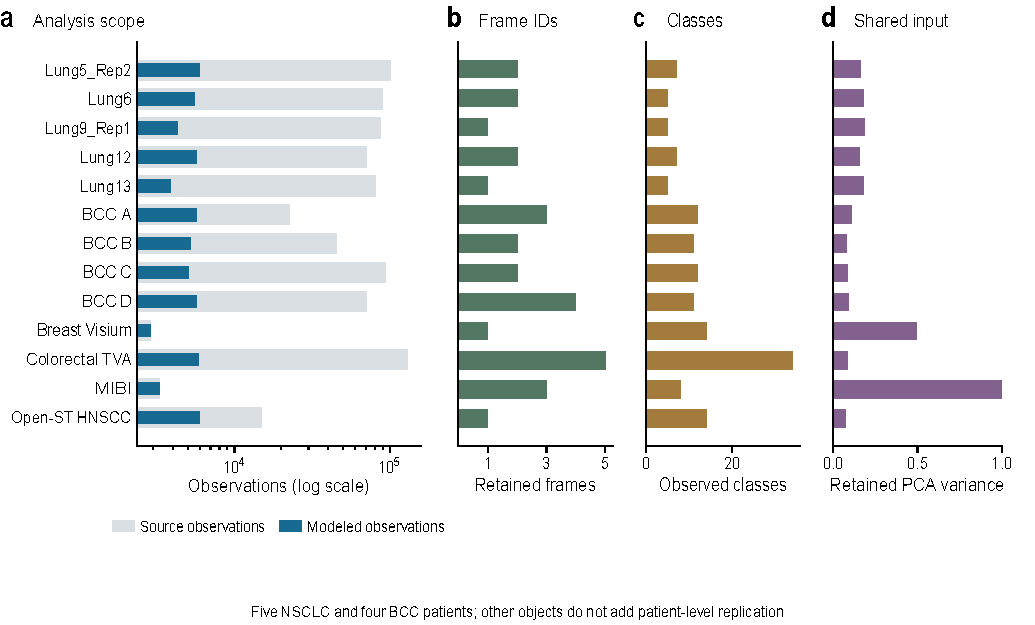
\includegraphics{journal-figures/figure02-cohort.pdf}
\caption{Scope of the bounded inputs. (a) Source and modeled observations on a logarithmic axis. (b) Retained coordinate frames. (c) Observed reference classes. (d) Fraction of total variance of the standardized, clipped input retained by the common 50-component PCA.}\end{figure}
\begin{figure}[p]\centering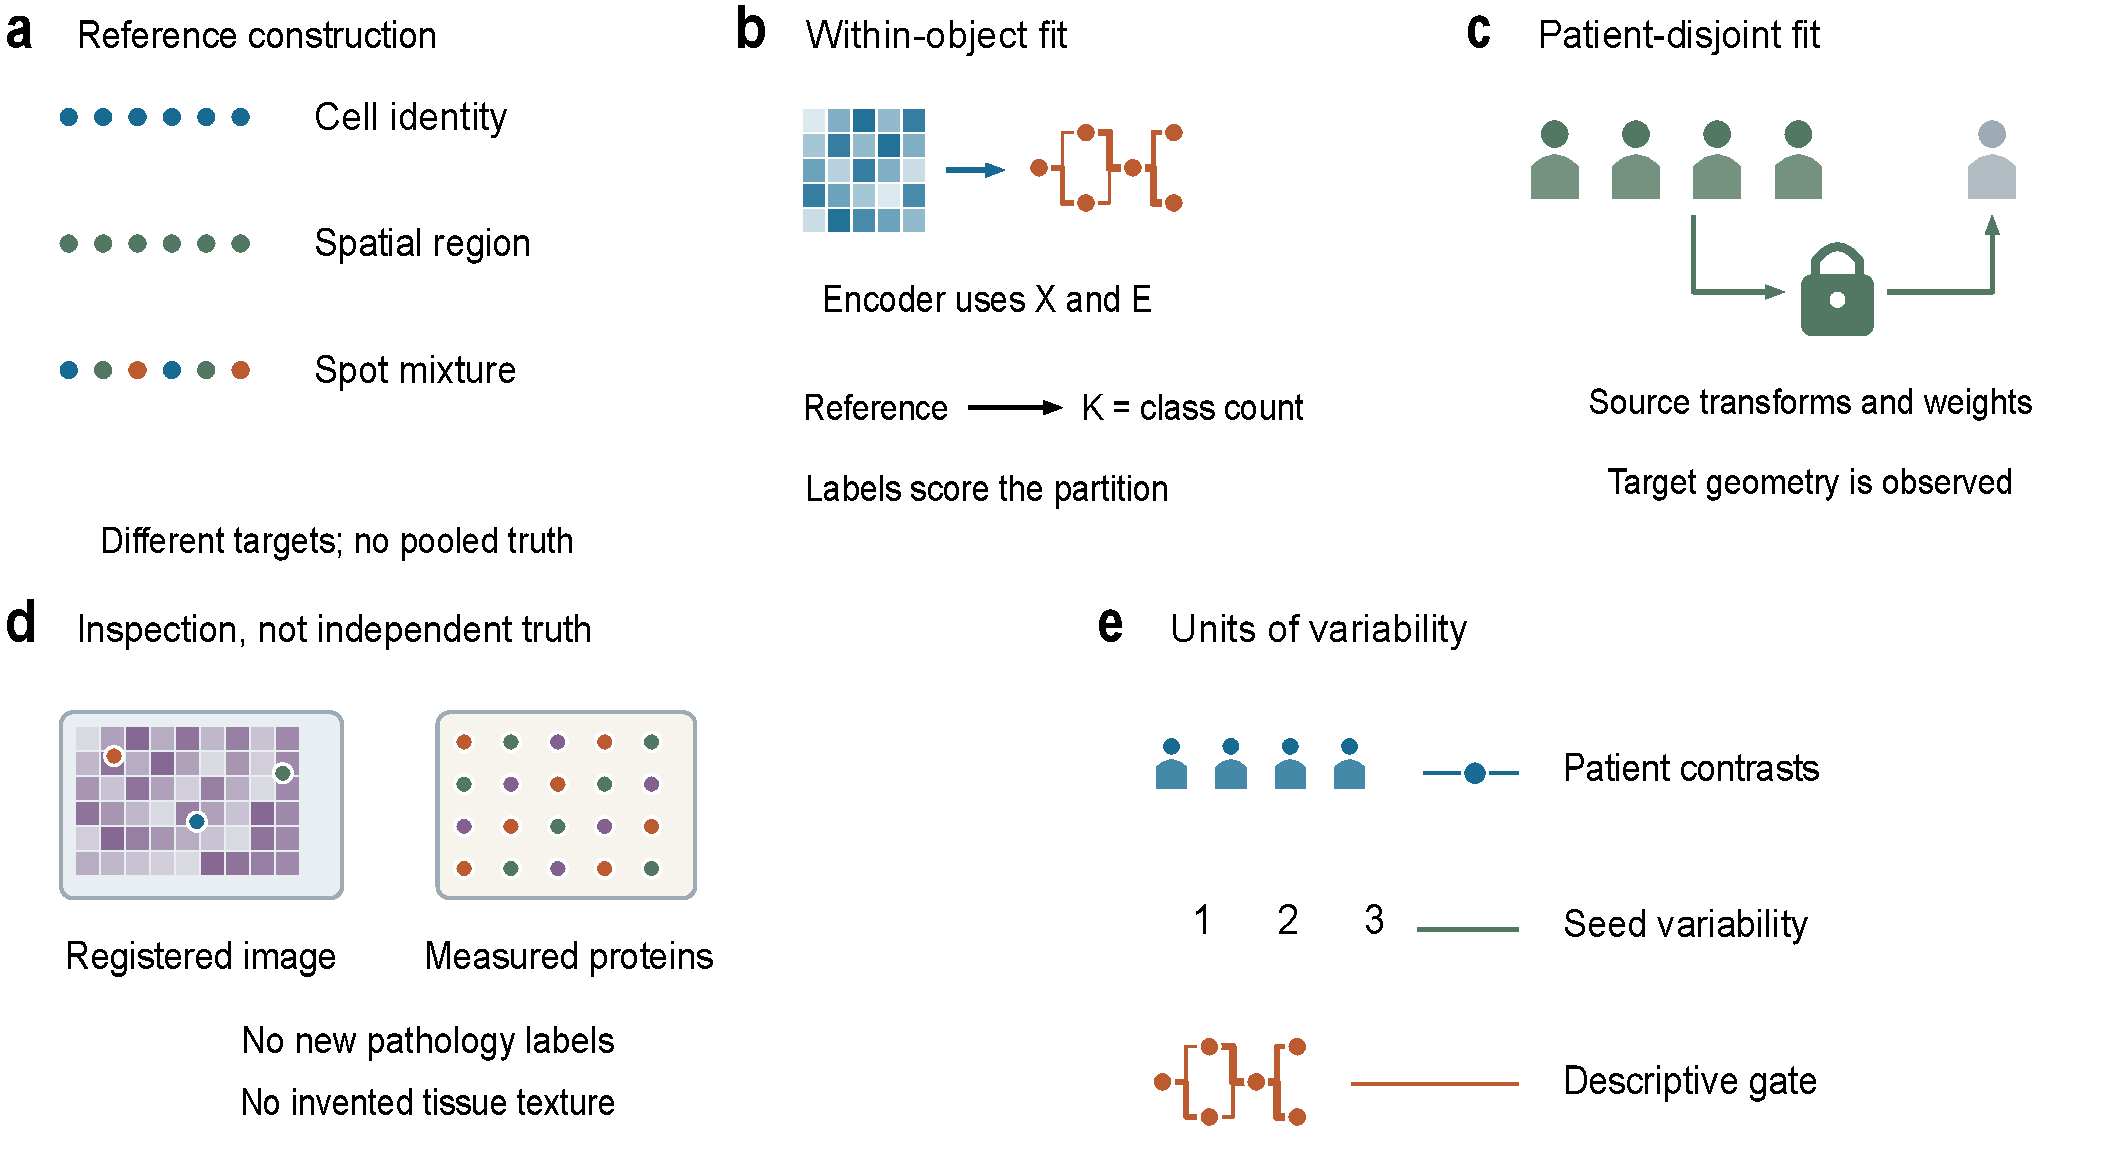
\includegraphics[width=\linewidth]{journal-figures/figure14-target-lineage.pdf}
\caption{Targets and information access, conceptual. (a) Molecular cell categories, neighborhood-derived regions and mixed-spot compositions come from different constructions. (b) Within-object clustering uses the reference class count but no reference labels. (c) Patient transfer freezes all fitted quantities before the held-out patient is mapped. (d) Registered images and protein channels support inspection only. (e) Patient contrasts, seed variation and gate readouts answer different questions.}\end{figure}
\begin{figure}[p]\centering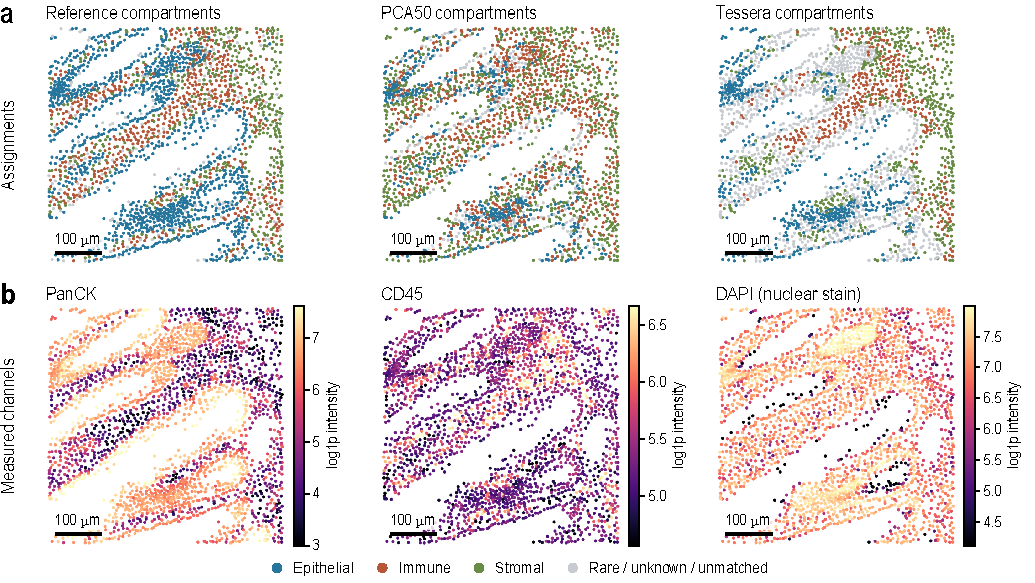
\includegraphics{journal-figures/figure09-colorectal-proteins.pdf}
\caption{Colorectal TVA section 232, display field. (a) Supplied compartments and display-matched PCA50 and Tessera assignments; only \texttt{lv2} classes with at least 1\% object prevalence are eligible for matching before modal compartment mapping, and unmatched clusters are gray. (b) Measured PanCK, CD45 and DAPI mean intensities, shown as \(\log(1+x)\) with field-wise 2nd--98th percentile color limits.}\end{figure}
\begin{figure}[p]\centering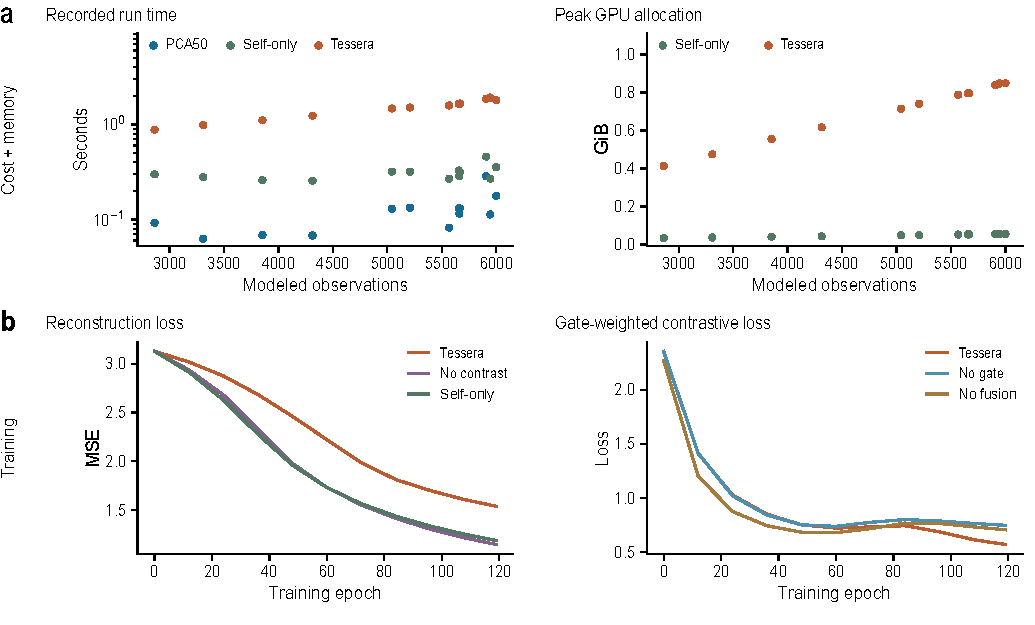
\includegraphics{journal-figures/figure12-efficiency-mechanism.pdf}
\caption{Execution and training records. (a) Recorded run time against modeled observations and peak GPU allocation. (b) Reconstruction and gate-weighted contrastive losses for Lung5\_Rep2, seed 1, at the saved epochs.}\end{figure}
\begin{figure}[p]\centering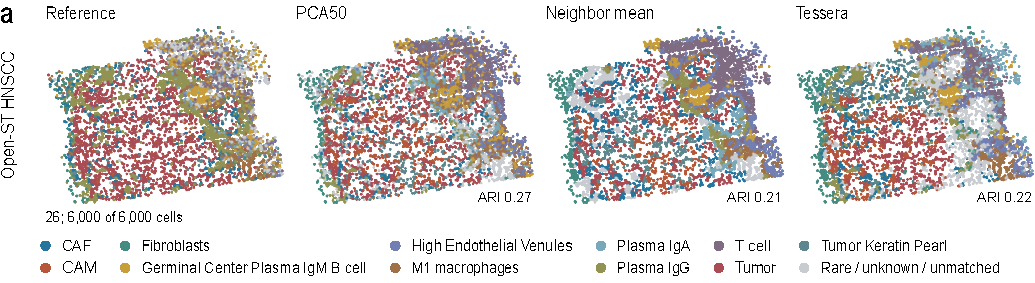
\includegraphics{journal-figures/supplement01-hnscc.pdf}
\caption{Open-ST section 26, complete selected 6,000-observation subset. (a) Supplied annotations, PCA50, the six-neighbor mean and Tessera on identical coordinates (seed 1). Matching excludes classes below 1\% object prevalence; rare reference labels, unknowns and unmatched clusters are gray. ARI badges retain original predictions and all valid classes, averaged over three seeds.}\end{figure}
\begin{figure}[p]\centering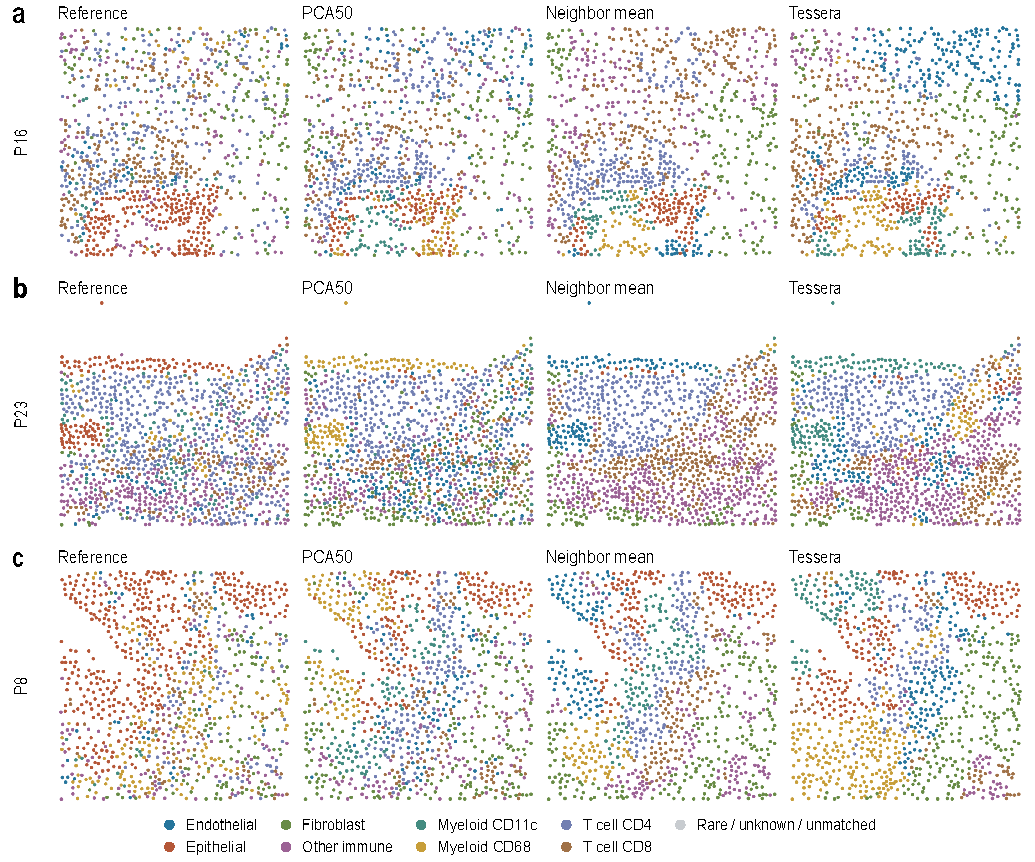
\includegraphics{journal-figures/supplement02-mibi.pdf}
\caption{Three MIBI fields in rows (a--c). Columns show supplied molecular categories, PCA50, the six-neighbor mean and Tessera (seed 1). Matching excludes reference classes below 1\% object prevalence; rare reference labels, unknowns and unmatched clusters are gray. Fields are not independent patients.}\end{figure}
\begin{figure}[p]\centering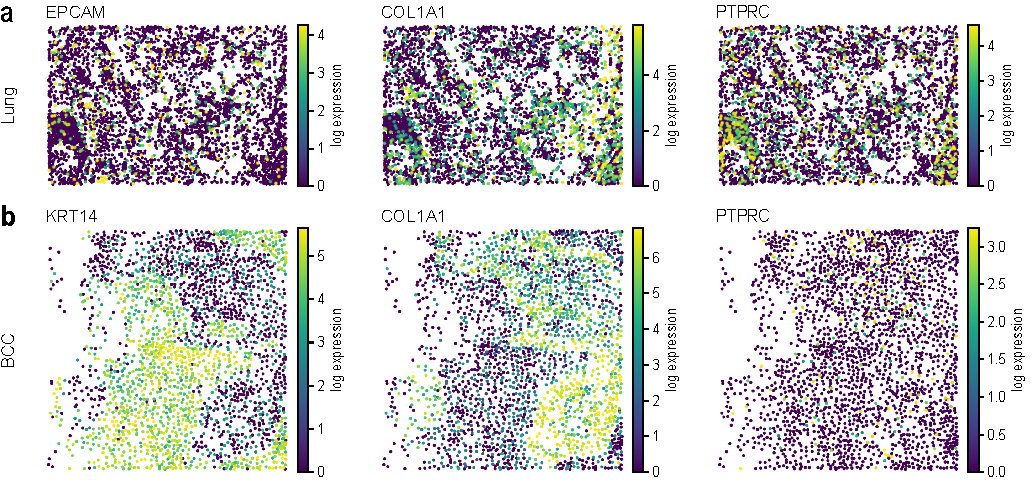
\includegraphics{journal-figures/supplement03-rna-markers.pdf}
\caption{Measured RNA markers in the display fields. (a) Lung EPCAM, COL1A1 and PTPRC. (b) BCC KRT14, COL1A1 and PTPRC. Values are the saved log-normalized expression with 0--98th percentile color limits; high-expressing cells are drawn on top.}\end{figure}
\begin{figure}[p]\centering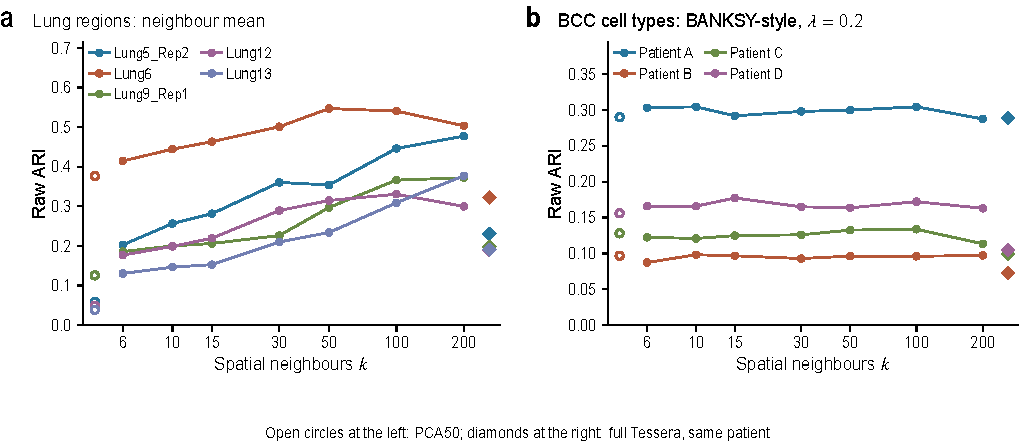
\includegraphics{journal-figures/supplement05-scale-controls.pdf}
\caption{Agreement of simple spatial controls as a function of neighborhood size. (a) Lung region ARI of the neighbor mean. (b) BCC cell-type ARI of the BANKSY-style representation with \(\lambda=0.2\). Each line is one patient (three-seed mean); open circles at the left mark PCA50 and diamonds at the right mark full Tessera for the same patient.}\end{figure}
\begin{figure}[p]\centering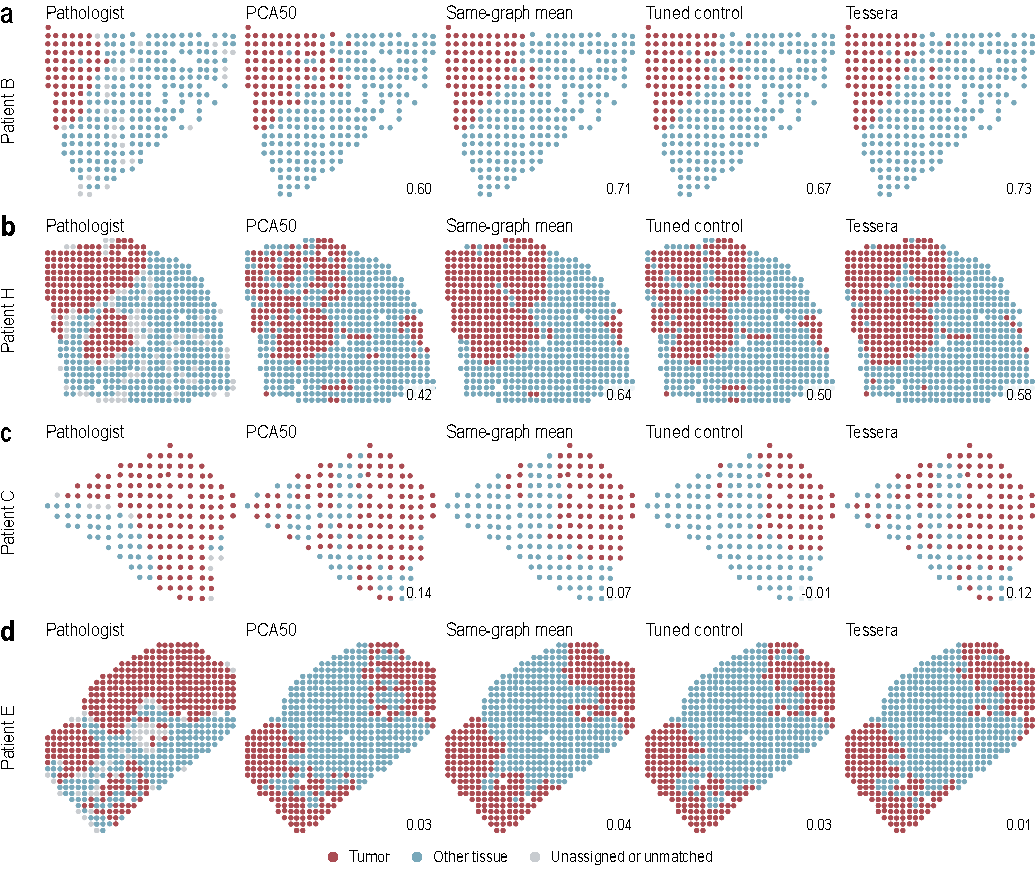
\includegraphics{journal-figures/figure16-external-maps.pdf}
\caption{Tumor boundary in four of the eight independent patients: rows (a--d) are the two patients with the highest (B, H) and the two with the lowest (C, E) same-graph mean agreement. Columns show the pathologist's regions, PCA50, the unweighted mean of neighbors on Tessera's graph, a tuned control selected on the other seven patients, and Tessera (seed 1). Clusters are matched to the two classes for display only; gray marks spots the pathologist left unassigned and unmatched clusters. Badges give the three-seed mean ARI against tumor versus other tissue.}\label{fig:externalmaps}\end{figure}

\clearpage\section*{Additional supporting displays}
\begin{figure}[htbp]\centering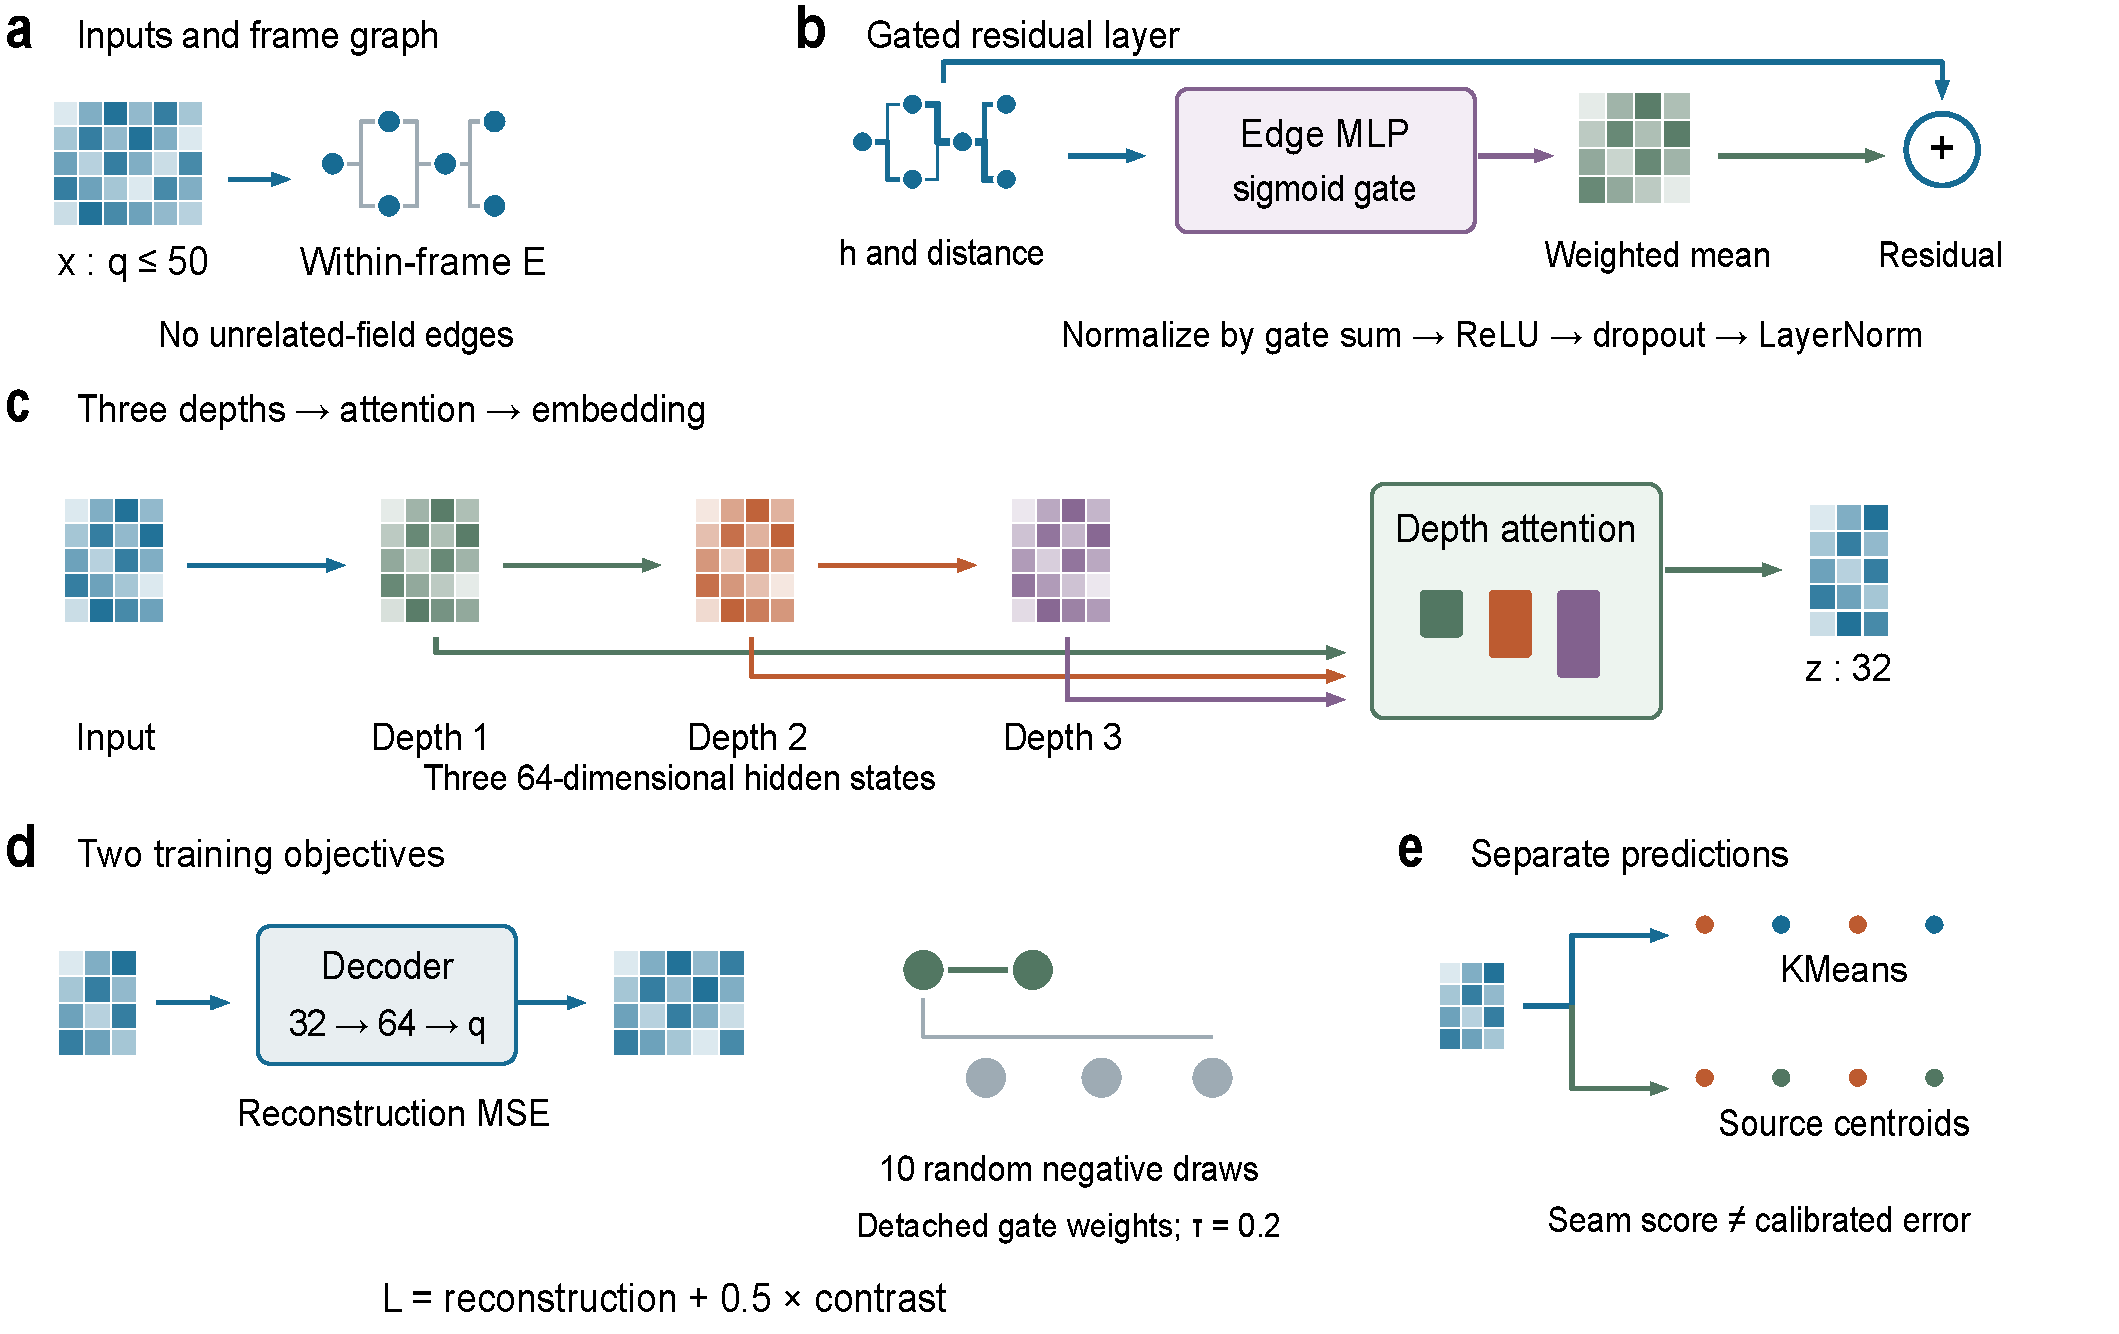
\includegraphics[width=\linewidth]{journal-figures/figure13-architecture.pdf}
\caption{The Tessera computation as released. (a) Common PCA features and frame-restricted neighborhoods. (b) Edge differences and distances determine gates; gated messages are normalized before a residual update. (c) Three depths feed attention and a 32-dimensional projection. (d) A decoder reconstructs the PCA features; neighbor-positive contrast is weighted by detached gates. (e) K-means returns the within-object partition, and source-category centroids return transfer labels. Glyphs are conceptual; dimensions are those implemented.}\label{fig:architecture}\end{figure}

\begin{table}[htbp]\centering\small
\caption{Three-seed mean ARI on the 13 objects with the primary cluster number. \(\Delta\) is Tessera minus PCA50.}\label{tab:results}
\begin{tabular}{lrrrrr}\toprule Object & PCA50 & Neighbor mean & Tessera & Self-only & $\Delta$\\\midrule
\tableinput ledgers/result_rows.tex
\bottomrule\end{tabular}\end{table}

\begin{table}[htbp]\centering\scriptsize\setlength{\tabcolsep}{4pt}
\caption{Tuned spatial controls and whole sections. Bounded-field controls maximize mean ARI over the other patients; values are three-seed means. Whole sections use all eligible cells and fixed cohort-modal controls (200-neighbor mean for NSCLC; BANKSY-style, \(k=100\), \(\lambda=0.2\) for BCC), informed by the bounded analysis of the same patients. Whole-section values are sensitivity results, not independently nested selections.}\label{tab:nested}
\begin{tabular}{llrrrrrrr}\toprule
& & \multicolumn{3}{c}{Bounded fields} & \multicolumn{4}{c}{Whole sections}\\\cmidrule(lr){3-5}\cmidrule(lr){6-9}
Patient & Selected control & PCA50 & Control & Tessera & Cells & PCA50 & Control & Tessera\\\midrule
\tableinput ledgers/followup_rows.tex
\bottomrule\end{tabular}\end{table}

\begin{figure}[htbp]\centering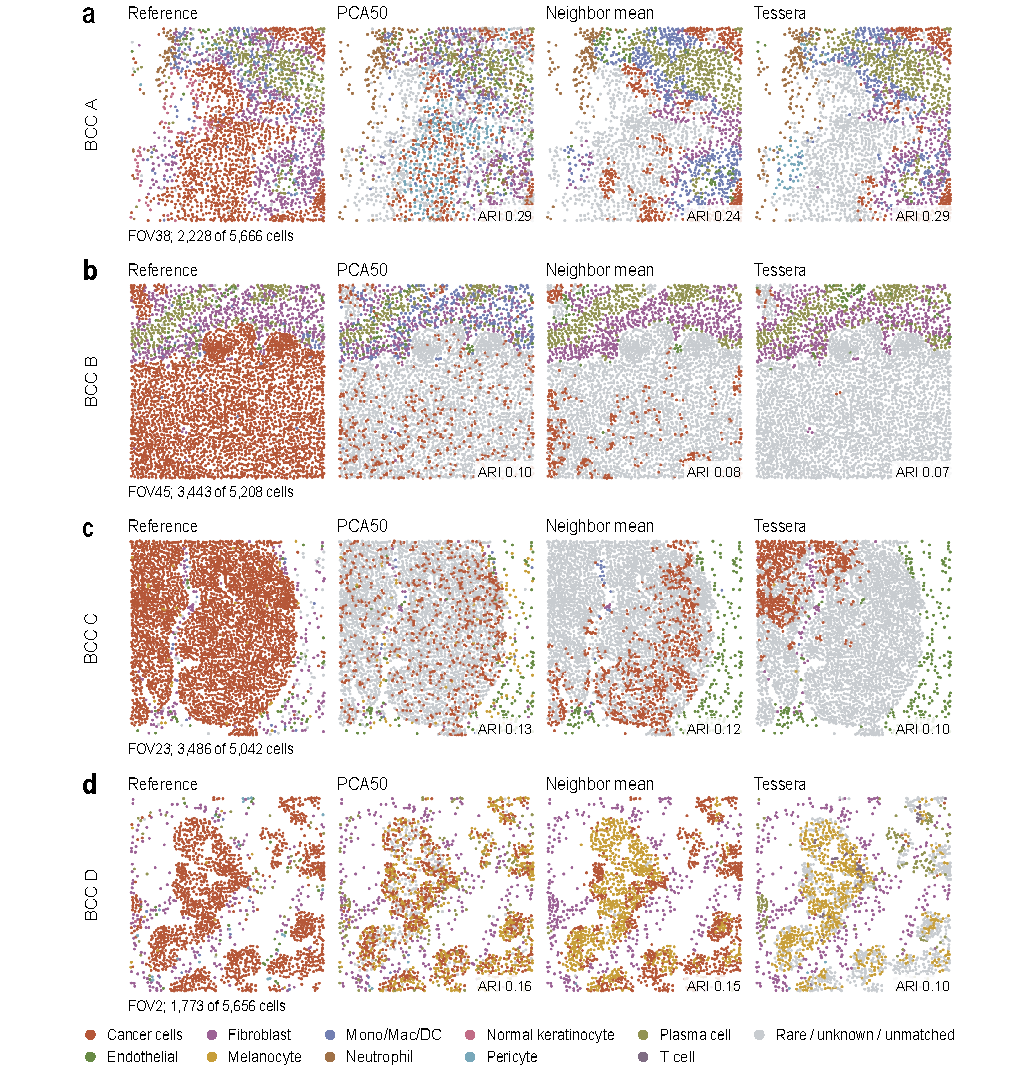
\includegraphics{journal-figures/figure06-bcc-maps.pdf}
\caption{BCC display fields. Rows (a--d) show Patients A--D; columns show supplied cell types, PCA50, the six-neighbor mean and Tessera. Seed-1 clusters are matched only to reference classes with at least 1\% object-level prevalence; rare reference classes, unknown labels and unmatched clusters are gray. ARI badges retain original predictions and all valid labels, averaged over three seeds and all retained fields.}\label{fig:bcc}\end{figure}

\begin{figure}[htbp]\centering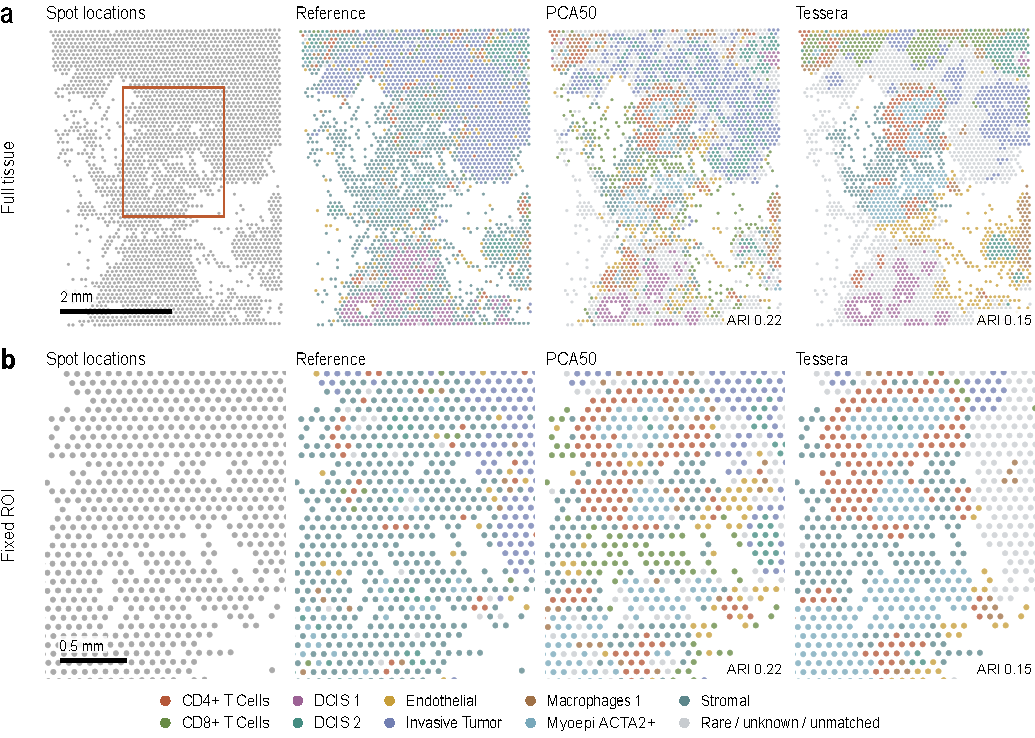
\includegraphics{journal-figures/figure07-breast-histology.pdf}
\caption{Breast spatial coordinates and matched representations. Row (a) shows full tissue and row (b) a median-centered ROI with fixed 22\% half-extent, chosen without labels or scores. Columns show measured spot locations, the dominant Xenium-derived reference, PCA50 and Tessera (seed 1). All panels are author-generated coordinate maps; no source histology image is reproduced. Matching excludes reference categories below 1\% object prevalence; rare reference labels, unknowns and unmatched clusters are gray. ARI badges retain all valid classes and are three-seed means. Scale bars use source calibration.}\label{fig:histology}\end{figure}

\begin{figure}[htbp]\centering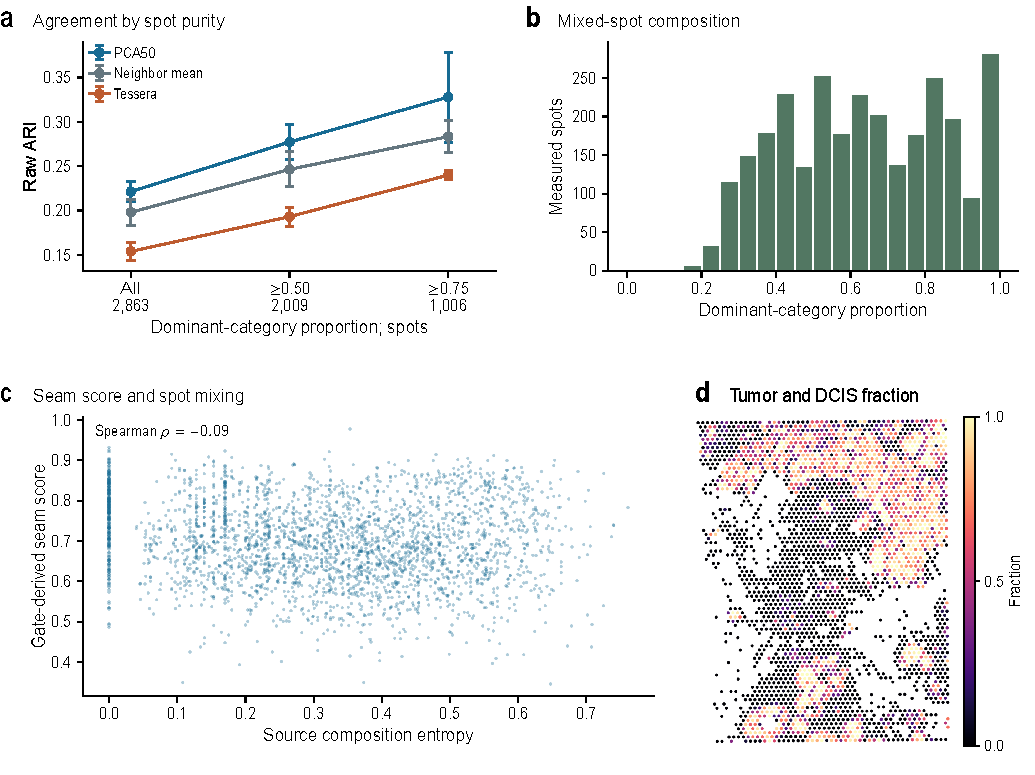
\includegraphics{journal-figures/figure08-breast-mixtures.pdf}
\caption{Breast mixed spots. (a) ARI of the fitted partitions when evaluation is restricted to spots whose dominant category exceeds 0.50 or 0.75; error bars are seed SD and the spot counts are under the axis. (b) Distribution of the dominant-category proportion. (c) Gate-derived seam score against source composition entropy (seed 1); a boundary-sensitive score would rise with mixing. (d) Supplied tumor and DCIS fraction per spot.}\label{fig:mixtures}\end{figure}

\begin{figure}[htbp]\centering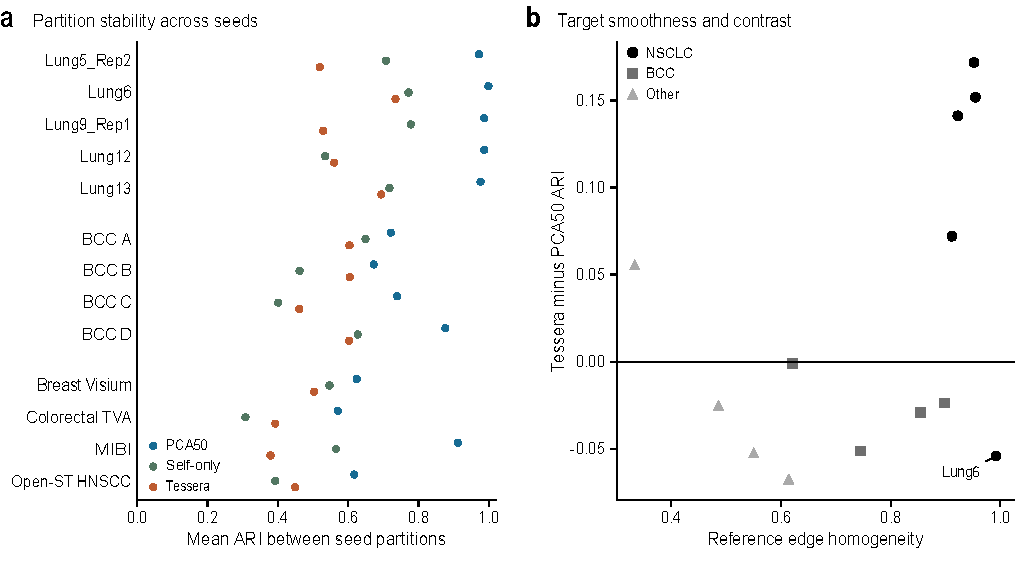
\includegraphics{journal-figures/figure11-stability.pdf}
\caption{Optimization stability and target structure. (a) Mean ARI between the three seed partitions on identical inputs. (b) Reference edge homogeneity, the fraction of spatial edges whose endpoints share a supplied label, against the Tessera minus PCA50 contrast. Lung6 is labelled because its high homogeneity reflects a display field dominated by one region.}\label{fig:stability}\end{figure}

\begin{table}[htbp]\centering\scriptsize\setlength{\tabcolsep}{3.6pt}
\caption{Independent pathologist cohort, three-seed mean ARI. The tuned control for each patient was selected on the other seven patients; the same-graph mean averages neighbors on Tessera's graph without tuning. Section identifiers are in parentheses; Classes counts the annotation classes scored for all labels.}\label{tab:external}
\begin{tabular}{lrrrrrrrrr}\toprule
& & & \multicolumn{4}{c}{All labels} & \multicolumn{3}{c}{Tumor boundary}\\\cmidrule(lr){4-7}\cmidrule(lr){8-10}
Patient & Spots & Classes & PCA50 & Same-graph mean & Tuned control & Tessera & Same-graph mean & Tuned control & Tessera\\\midrule
\tableinput ledgers/external_rows.tex
\bottomrule\end{tabular}\end{table}
\end{document}
